\begin{center}
    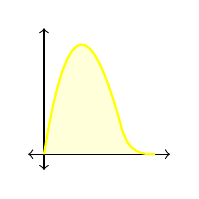
\begin{tikzpicture}
        \fill[color=Yellow!15, thick, domain=0:1.412136] plot (\x, {(\x <= 1) * (2 * pi * \x - 8 * \x^2 + 2 * \x^3) + (\x > 1) * (2 * pi * \x - 2 * \x^3 - 4 * \x + 8 * \x * sqrt(abs(\x^2 - 1)) - 8 * \x * rad(atan(sqrt(abs(\x^2 - 1)))))}) -- (0, 0) -- cycle;

        \draw[<->] (-0.2, 0) -- (1.6, 0);
        \draw[<->] (0, -0.2) -- (0, 1.6);

        \draw[color=Yellow, thick, domain=0:1.412136] plot (\x, {(\x <= 1) * (2 * pi * \x - 8 * \x^2 + 2 * \x^3) + (\x > 1) * (2 * pi * \x - 2 * \x^3 - 4 * \x + 8 * \x * sqrt(abs(\x^2 - 1)) - 8 * \x * rad(atan(sqrt(abs(\x^2 - 1)))))});
    \end{tikzpicture}
\end{center}
\captionof{figure}{The final distribution and the distribution of all distances
between two points found on the unit square. This particular distribution has a
somewhat intuitive shape. Note however that the mean is not extreme value,
although they look somewhat close.}
